%% We use `subfiles' package
\documentclass[preamble.tex]{subfiles}
\begin{document}


\clearpage

\chapter{Results}
\label{ch:results}


\section{QuickHull}
\label{sec:quickhull}

\begin{figure}
\includegraphics[center]{img/Example-QH1000}
\end{figure}

\subsection{The heart of QuickHull}

\subsection{Segmented FilterMax}

\subsection{Evaluation}

\begin{figure}
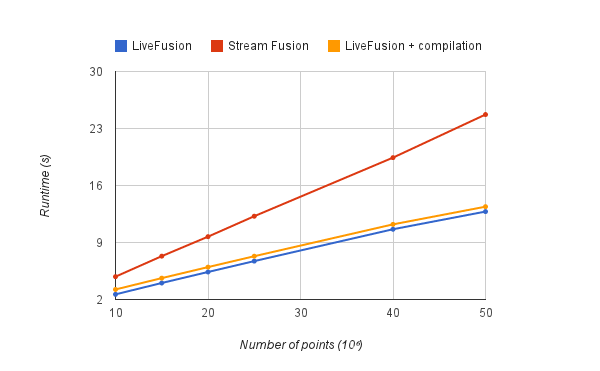
\includegraphics[center]{img/Eval-QuickHull}
\end{figure}

\begin{figure}
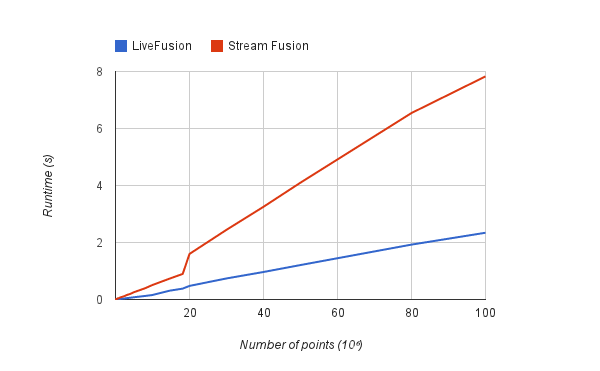
\includegraphics[center]{img/Eval-FarAndAboves}
\end{figure}

\begin{figure}
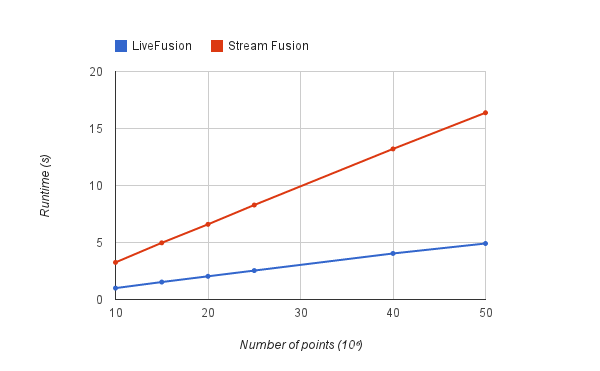
\includegraphics[center]{img/Eval-FarAndAboves-Overall}
\end{figure}

\clearpage
\section{Compilation time and amortisation}


\IfNotCompilingAll{\bibliography{bib}}

\end{document}